\documentclass[a4paper,11pt]{report}
\usepackage{booktabs}
\renewcommand{\arraystretch}{1.3}
%-------------------------------------------------------------------------------
%	FONT
%-------------------------------------------------------------------------------
\usepackage[utf8]{inputenc}
\usepackage[T1]{fontenc}

%\usepackage[scaled=0.8]{beramono} % beramono or luximono give very nice ttfamily fonts

%-------------------------------------------------------------------------------
%	PAGE LAYOUT
%-------------------------------------------------------------------------------
\usepackage[toc,page]{appendix}

\textwidth = 410pt

\usepackage{fancyhdr}
\pagestyle{fancy}
\fancyhf{}

%\renewcommand{\sectionmark}[1]{\markright{\thesection.\ #1}}

%\nouppercase{\rightmark}

\lhead{\bfseries \nouppercase{\leftmark}}
\rhead{\bfseries \nouppercase{\rightmark}}
\lfoot{}
\rfoot{\bfseries Page \thepage}

\headwidth=1.1\textwidth
\renewcommand{\headrulewidth}{1.5pt}
\renewcommand{\footrulewidth}{1.5pt}
\fancyhfoffset[L]{24pt}
\fancyhfoffset[R]{24pt}

\fancypagestyle{plain}{%
\fancyhf{} % clear all header and footer fields
\headwidth=1.1\textwidth
\renewcommand{\headrulewidth}{1.5pt}
\renewcommand{\footrulewidth}{1.5pt}
\lhead{\bfseries \nouppercase{\leftmark}}
\rhead{\bfseries \nouppercase{\rightmark}}
%\lhead{\leftmark}
%\rhead{\rightmark}
\lfoot{}
\rfoot{\bfseries Page \thepage}
%\rfoot{Page \thepage}
\headwidth=1.1\textwidth
\fancyhfoffset[L]{24pt}
\fancyhfoffset[R]{24pt}
}

\newcommand{\mysection}[2]{%
                         \sectionmark{#1}%
                         \section{#2}%
                         \sectionmark{#1}%
                       }

%%%%%%%%%
%\renewcommand{\chaptermark}[1]{\markboth{\uppercase{\thechapter.\ #1}}{}}
%\renewcommand{\sectionmark}[1]{\markright{\uppercase{\thesection.\ #1}}}
%\newcommand{\helv}{\fontfamily{phv}\fontseries{b}\fontsize{9}{11}\selectfont}
%\lhead[\helv \thepage]{\helv \rightmark}
%\rhead[\helv \leftmark]{\helv \thepage}
%\cfoot{}
%-------------------------------------------------------------------------------
%	OTHER PACKAGES and COMMANDS
%-------------------------------------------------------------------------------
\usepackage{graphicx}
\usepackage{epstopdf}


\usepackage{float}
\usepackage{tikz}
\usepackage{tikz-uml} 
\usepackage{amsmath}

\usepackage{pifont}
\usepackage{fourier}
\usepackage{dingbat}

\usepackage{hyperref}
\usepackage{breakurl}

\newcommand{\reffig}[1]{figure \ref{fig:#1}}

\newcommand{\myparagraph}[1]{\paragraph{#1}\mbox{}\\}
%-------------------------------------------------------------------------------
%	CUSTON LISTING SETTINGS
%-------------------------------------------------------------------------------
\usepackage{listings}
\usepackage{lstcustom}
\usepackage{enumerate}
\renewcommand{\lstfontfamily}{\ttfamily}
%-------------------------------------------------------------------------------
%	COLORS
%-------------------------------------------------------------------------------

\definecolor{Lightgray}{gray}{.80}
\definecolor{lightgrey}{rgb}{0.9,0.9,0.9}


%-------------------------------------------------------------------------------
%       Commands
%-------------------------------------------------------------------------------
\newcommand{\Code}[1]{\texttt{#1}}
\newcommand{\BornAgain}{\Code{BornAgain}}%
\newcommand{\IsGISAXS}{\Code{IsGISAXS}}%
\newcommand{\SecLabel}[1]{\label{sec:#1}}%
\newcommand{\SecRef}[1]{Section~\ref{sec:#1}}% 
\newcommand{\MakeRemark}[2]
{ \noindent \smallpencil \colorbox{Lightgray}{\parbox{\dimexpr\linewidth-8\fboxsep}			{\underline{#1} #2 }}
}

\newcommand{\ImportantPoint}[2]
{\noindent
  {\huge\danger}\colorbox{Lightgray}{\parbox{\dimexpr\linewidth-8\fboxsep}
 {\underline{#1} #2}}}

\newcommand{\mychapter}[2]{
    \setcounter{chapter}{#1}
    \setcounter{section}{0}
    \chapter*{#2}
    \addcontentsline{toc}{chapter}{#2}
}

%-------------------------------------------------------------------------------
%	TITLE PAGE
%-------------------------------------------------------------------------------
\title{
{\Huge\bf BornAgain}\\[10mm]
Software for simulating and fitting\\
X-ray and neutron small-angle scattering\\
at grazing incidence\\
\vspace*{10mm} User Manual \\
\large{version 0.1.1\\\today}
\vspace*{5mm}
}

\author{ 
{\LARGE C. Durniak, G. Pospelov, W. Van Herck, J. Wuttke }\\[5mm]
\large
Scientific Computing Group\\
J\"ulich Centre for Neutron Science\\
outstation at Heinz Maier-Leibnitz Zentrum Garching\\
Forschungszentrum J\"ulich GmbH
}

\date{{}}
%License: Creative Common CC-BY-SA \\
%\today
%}


%\usepackage{eso-pic}
%\newcommand\BackgroundPic{%
%\put(0,0){%
%\parbox[b][\paperheight]{\paperwidth}{%
%\vfill
%\centering
%\includegraphics[width=\paperwidth,height=\paperheight,%
%keepaspectratio]{results2_2.png}%
%\vfill
%}}}


%-------------------------------------------------------------------------------
%	DOCUMENT
%-------------------------------------------------------------------------------
\begin{document}

\maketitle


\newpage

{\Huge 
\vspace*{0.5cm}
\noindent
Disclaimer
} \newline
\vspace*{0.25cm}

\noindent
{\large
This manual supplements BornAgain online documentation located at \url{http://www.bornagainproject.org}.
Follow the link to get started.
\vspace*{4mm}

\noindent
This manual is under development and does not yet constitute a comprehensive listing of
all \BornAgain\ features and functionality. 
The included information and instructions are subject to substantial changes and
are provided only as a preview.
}

\tableofcontents
%\lstlistoflistings
%\listoffigures
%\listoftables
%%%%%%%%%%%%%%%%%%%%%%%%%%%%%%%%%%%%%%%%%%%%%%%%%%%%%%%%%%%%%%%%%%%%%%%%%%%%%%%%
%%
%%   BornAgain User Manual
%%
%%   homepage:   http://www.bornagainproject.org
%%
%%   copyright:  Forschungszentrum Jülich GmbH 2015
%%
%%   license:    Creative Commons CC-BY-SA
%%
%%   authors:    Scientific Computing Group at MLZ Garching
%%               C. Durniak, M. Ganeva, G. Pospelov, W. Van Herck, J. Wuttke
%%
%%%%%%%%%%%%%%%%%%%%%%%%%%%%%%%%%%%%%%%%%%%%%%%%%%%%%%%%%%%%%%%%%%%%%%%%%%%%%%%%


\cleardoublepage
\ichapter{Introduction}

%%%%%%%%%%%%%%%%%%%%%%%%%%%%%%%%%%%%%%%%%%%%%%%%%%%%%%%%%%%%%%%%%%%%%%%%%%%%%%%%
\isection{About BornAgain}
%%%%%%%%%%%%%%%%%%%%%%%%%%%%%%%%%%%%%%%%%%%%%%%%%%%%%%%%%%%%%%%%%%%%%%%%%%%%%%%%

\BornAgain\ is a software package
to simulate and fit
reflectometry, off-specular scattering,
and grazing-incidence small-angle scattering (GISAS)
of X-rays and neutrons.
It provides a generic framework
for modeling multilayer samples with smooth or
rough interfaces and with various types of embedded nanoparticles.
Support for neutron polarization and magnetic scattering
is under development.
The name, \BornAgain,
alludes to the central role of the distorted-wave Born
approximation (DWBA) in the physical description of the
scattering process.
\index{Distorted-wave Born approximation}

\BornAgain\ is being developed
by the Scientific Computing Group
of the J\"ulich Centre for Neutron Science (JCNS)
at Heinz Maier-Leibnitz Zentrum (MLZ) Garching, Germany.
It is intended to serve experimentalists in analysing all kinds
of reflectometry data.
It is equally aimed at users of MLZ reflectometers
\cite{mlz:maria,mlz:nrex,mlz:refsans},
at JCNS in-house researchers,
and at the reflectometry and GISAS community at large.
It is the main contribution of JCNS to national \cite{ba:hdri}
and international \cite{ba:sine2020} collaborations
of large-scale facilities for the development of better user software.

\BornAgain\ is released as free and open source software under
the GNU General Public License (GPL, version 3 or higher).
This documentation comes under the Creative Commons license CC-BY-SA.

\Warn{\indent The converse of this liberal policy is
that we cannot guarantee correctness and accuracy of the code.
It is entirely in the responsibility of users
to convince themselves that their data interpretation
is physically meaningful and plausible.}
\Work{\indent\BornAgain\ is still under intense development.
New major versions are released about every few months.
When need arises, bugfix versions are released in between.
It is strongly recommended that users regularly update their installations.}

The software \BornAgain\ embodies nontrivial scientific ideas.
Therefore when \BornAgain\ is used in preparing scientific papers,
it is mandatory to cite the software:
\index{Citation}%
%\marginpar{citation}%
\begin{quote}
\authors\ (2013--\the\year),\newline
BornAgain --- Software for simulating and fitting
X-ray and neutron small-angle scattering at grazing incidence,
version [\ldots],\newline
\url{http://www.bornagainproject.org}
\end{quote}
The initial design of \BornAgain\ owes much
to the widely used program \IsGISAXS\
\index{IsGISAXS@\IsGISAXS}%
\index{Lazzari, R\'emi}%
by R\'emi Lazzari \cite{Laz02,Laz08}.
Therefore when using \BornAgain\ in scientific work,
it might be appropriate to also cite the pioneering papers
by Lazzari \etal\ \cite{Laz02,ReLL09}.

Since version 1.0, \BornAgain\
almost completely reproduces the functionality
of \IsGISAXS.
About 20 exemplary simulations have been tested against \IsGISAXS,
and found to agree up to almost the last floating-point digit.
\BornAgain\ goes beyond \IsGISAXS\
in supporting an unrestricted number of layers and particles,
diffuse reflection from rough layer interfaces and
particles with inner structures.
Support for neutron polarization and magnetic scattering
is under development.
Adhering to a strict object-oriented design,
\BornAgain\ provides a solid base for future extensions
in response to specific user needs.

%%%%%%%%%%%%%%%%%%%%%%%%%%%%%%%%%%%%%%%%%%%%%%%%%%%%%%%%%%%%%%%%%%%%%%%%%%%%%%%%
\isection{Registration, contact, discussion forum}\label{Snews}
%%%%%%%%%%%%%%%%%%%%%%%%%%%%%%%%%%%%%%%%%%%%%%%%%%%%%%%%%%%%%%%%%%%%%%%%%%%%%%%%

\index{Registration}
\index{Newsletter}
To stay informed about the ongoing development of \BornAgain,
register on the project homepage \url{http://www.bornagainproject.org}
(``Create new account'').
You will then receive our occasional newsletters,
and be authorized to post to the discussion forum.

\index{Contact}
To contact the \BornAgain\ development and maintenance team
in the Scientific Computing Group
of Heinz Maier-Leibnitz Zentrum (MLZ) Garching,
write a mail to \url{contact@bornagainproject.org},
or fill the form in the \textsc{Contact} section of the
project web site.

\index{Forum}
For questions that might be of wider interest,
please consider posting to the discussion forum,
accessible through the \textsc{Forums} tab of the project web site.

\index{Bug reports}%
Please contact us for any question not answered here
or in the online documentation.
We are grateful for all kind of feedback:
criticism, praise, bug reports, feature requests or contributed modules.
If questions go beyond normal user support,
we will be glad to discuss a scientific collaboration.

%%%%%%%%%%%%%%%%%%%%%%%%%%%%%%%%%%%%%%%%%%%%%%%%%%%%%%%%%%%%%%%%%%%%%%%%%%%%%%%%
\isection{About this Manual}
%%%%%%%%%%%%%%%%%%%%%%%%%%%%%%%%%%%%%%%%%%%%%%%%%%%%%%%%%%%%%%%%%%%%%%%%%%%%%%%%

This User Manual is complementary to the online documentation
at \url{http://www.bornagainproject.org}.
It does not duplicate information that is more conveniently read online.
The online documentation covers in particular
how to download and install \BornAgain.

This User Manual containes of two parts:
\Cref{PPHYS} provides physics background
on the scattering theory and on the sample models implemented in \BornAgain.
\cref{PREF} is a partial reference of the C$++$ and Python interfaces;
it concentrates on physics related component,
and thereby complements the automatically generated interface documentation
that can be found online at \url{http://apps.jcns.fz-juelich.de/doxy/BornAgain/index.html}.

\Work{\indent This manual is incomplete.
Several important chapters are still incomplete, or only consist of a placeholder.}
We intend to publish the missing material successively,
along with new software release.

\pagebreak[3]
We use the following colored boxes to highlight
certain information:

\def\demobox#1{\noindent\strut\hspace{.2\TW}\begin{minipage}{.75\textwidth}#1
\end{minipage}\hfill\strut}

\medskip
\demobox{\Warn{\indent Such a box contains
a \textbf{warning} about potential problems
with the software or the documentation.}}

\medskip
\demobox{\Work{\indent This road sign in the margin indicates \textbf{work in progress}.}}

\medskip
\demobox{\Emph{\indent A green box highlights
  an \textbf{important fact}, for instance an equation
  that is central in
  the further development of the theory.}}

\medskip
\demobox{\Note{\indent
  An \textbf{implementation note} explains
  how the theory exposed in this manual is actually used in \BornAgain.}}

\medskip
\noindent\strut\hspace{.2\TW}This is a \tuto{1}{link to the online docs}.

\medskip
\setCpp
\begin{lstlisting}[linewidth=.95\TW,xleftmargin=.2\TW]
C++ code, mainly used for API documentation.
\end{lstlisting}

\setPy
\begin{lstlisting}[linewidth=.95\TW,xleftmargin=.2\TW]
Python code.
\end{lstlisting}

\bigskip
Mathematical notations are explained in the symbol index, page~\pageref{Snomencl}.

\newpage
\section{Quick start} \SecLabel{QuickStart}

This section shortly describes how to build \BornAgain\ from source and run first
simulation. More details about software architecture and installation
procedure are given in \SecRef{SoftwareArchitecture} and \SecRef{InstallationProcedure}. \\

\noindent
{\bf Step I: $~$ installing third party software}
\begin{itemize}
\item boost library ($\geq 1.48$)
\item GNU scientific library ($\geq 1.15$)
\item fftw3 library ($\geq 3.3.1$)
\item python-2.7, python-devel, python-numpy-devel
\item Eigen3 library ($\geq 3.1.0$), optional
\item ROOT framework ($\geq 5.34.00$), optional
\item python-matplotlib, optional
\end{itemize}
\vspace*{2mm}


\noindent
{\bf Step II: $~$ getting the source}
\begin{lstlisting}[language=bash, style=commandline]
git clone git://apps.jcns.fz-juelich.de/BornAgain.git 
\end{lstlisting}
\vspace*{3mm}


\noindent
{\bf Step III: $~$ building the source}
\begin{lstlisting}[language=shell, style=commandline]
mkdir <build_dir>; cd <build_dir>;
cmake <source_dir> -DCMAKE_INSTALL_PREFIX=<install_dir>
make
make check
make install
\end{lstlisting}
\vspace*{3mm}


\noindent
{\bf Step IV: $~$ running example}
\begin{lstlisting}[language=shell, style=commandline]
cd <install_dir>/Examples/python/ex001_CylindersAndPrisms
python CylindersAndPrisms.py
\end{lstlisting}


%Requirements

%Hardware
%BornAgain is known to work on following platforms:
%Linux (x86, amd64)
%MacOS X (x86)

%Software
%GCC 4.1.2 or above   C/C++ compiler
%or
%clang
%gcc 4.1.2 or above, clang

\newpage
\section{Installation} \SecLabel{installation}

This section shortly describes how to build \BornAgain\ from source and run first
simulation.

%%%%%%%%%%%%%%%%%%%%%%%%%%%%%%%%%%%%%%%%%%%%%%%%%%%%%%%%%%%%%%%%%%%%%%%%%%%%%%%
%
%%%%%%%%%%%%%%%%%%%%%%%%%%%%%%%%%%%%%%%%%%%%%%%%%%%%%%%%%%%%%%%%%%%%%%%%%%%%%%%


%\mysection{Example 1}{Example 1: two types of islands on top of
%  substrate without interference.} \SecLabel{Example1Python}

\section{Example 1: two types of islands on top of
  substrate without interference.} \SecLabel{Example1Python}

% \sectionmark{Example 1}

In this example, we simulate the scattering from a mixture of
cylindrical and prismatic nanoparticles without any interference
between them. These particles are placed in air, on top
of a substrate.\\ We are going to go through each step of the
simulation. The Python script specific to each stage will be given at
the beginning of the description. But for the sake of completeness the full code is given
at the end of this section (Listing~\ref{script_ex1}). \\

\noindent We start by importing different functions from external
modules (line~\ref{import_lib}), for example NumPy, which
is a fundamental package for scientific computing with Python \cite{s:numpy}.  In particular, line~\ref{import_end}
imports the features of \BornAgain\ software.\\

\begin{lstlisting}[language=python, style=eclipseboxed,name=ex1,nolol]
import sys, os, numpy @\label{import_lib}@

from libBornAgainCore import * @\label{import_end}@
\end{lstlisting}


 %%%%%%%%%%%%%  
\myparagraph{\underline{First step:} Defining materials} 
 

\begin{lstlisting}[language=python, style=eclipseboxed,name=ex1,nolol]
def RunSimulation(): @\label{def_function}@
    #  defining materials @\label{material1}@
    mAmbience = MaterialManager.getHomogeneousMaterial("Air", 0.0, 0.0)  @\label{material2}@
    mSubstrate = MaterialManager.getHomogeneousMaterial("Substrate",
    6e-6, 2e-8) @\label{material3}@
    mParticle = MaterialManager.getHomogeneousMaterial("Particle", 6e-4,
  2e-8 ) @\label{materialparticle}@
\end{lstlisting}

\noindent Line~\ref{def_function} marks the beginning of the
function to define and run the simulation. 

\noindent Lines~\ref{material2}, \ref{material3} and \ref{materialparticle} define different
materials using function \Code{getHomogeneousMaterial} from class
\Code{MaterialManager}. The general syntax is the following 

\begin{lstlisting}[language=python, style=eclipse,numbers=none]
<material_name> = MaterialManager.getHomogeneousMaterial("name", delta, beta)
\end{lstlisting}

\noindent where \Code{name} is the name of the
material associated with its complex refractive index
n=1-\Code{delta} +i \Code{beta}. \Code{<material\_name>} is later used when
referring to this particular material. The three defined materials in this example are \Code{Air} with a refractive
index of 1 (\Code{delta = beta =0}), a \Code{Substrate} associated with a complex refractive index
equal to $1-6\times 10^{-6} +i2\times 10^{-8} $, and the material of particles, whose refractive index is \Code{n}$=1-6\times 10^{-4}+i2\times 10^{-8}$.\\\\

%\noindent \underline{Remark:} there is no condition on the choice of \Code{name}. 
 %%%%%%%%%%%%% 
\myparagraph{\underline{Second step:} Defining the particles} 

\begin{lstlisting}[language=python,style=eclipseboxed,name=ex1,nolol]
    # collection of particles @\label{particles1}@
    cylinder_ff = FormFactorCylinder(5*nanometer, 5*nanometer) @\label{particlescyl1}@
    cylinder = Particle(mParticle, cylinder_ff) @\label{particlescyl2}@
    prism_ff = FormFactorPrism3(5*nanometer, 5*nanometer) @\label{particlesprism1}@
    prism = Particle(mParticle, prism_ff) @\label{particlesprism2}@
\end{lstlisting}

 \noindent We implement two different shapes of particles: cylinders and
 prisms (\textit{i.e.} elongated particles with a constant equilateral triangular cross section).\\ All particles implemented in \BornAgain\ are defined by their
 form factors, their sizes and the material
  they are made of. Here, for the
  cylindrical particle, we input its radius and height.  For the prism, 
  the possible inputs are the length of one side of its equilateral triangular
  base and its height.\\

%\noindent In line~\ref{complx_ref_index}, we define the complex refractive index
%associated with both particle shapes: \Code{n}$=1-6\times 10^{-4}+i2\times 10^{-8}$.\\
  
\noindent In order to define a particle, we proceed in two steps. For example for
the cylindrical particle, we first specify the form factor of a cylinder with 
its radius and height, both equal to 5 nanometers in this particular
case (see line~\ref{particlescyl1}). Then we associate this shape with
the constituting material as in line~\ref{particlescyl2}.\\

\noindent The same procedure has been applied for the prism in lines~\ref{particlesprism1} and \ref{particlesprism2} respectively.
 %%%%%%%%%%%%% 
\myparagraph{\underline{Third step:} Characterizing the layers and assembling the sample} 

\noindent \textbf{Particle decoration} \\
  

\begin{lstlisting}[language=python, style=eclipseboxed, name=ex1,nolol]
    particle_decoration = ParticleDecoration()  @\label{particlesdecor1}@
    particle_decoration.addParticle(cylinder, 0.0, 0.5)  @\label{particlesdecor2}@
    particle_decoration.addParticle(prism, 0.0, 0.5)@\label{particlesdecor3}@
    interference = InterferenceFunctionNone()  @\label{particlesnointerf}@
    particle_decoration.addInterferenceFunction(interference)  @\label{particlesinterf}@
\end{lstlisting}

\noindent The object which holds the information about the positions and densities of particles
in our sample is called \Code{ParticleDecoration}
(line~\ref{particlesdecor1}). We use the associated function \Code{addParticle}
for each particle shape (lines~\ref{particlesdecor2}, \ref{particlesdecor3}). Its general
syntax is 

\begin{lstlisting}[language=python, style=eclipse,numbers=none]
addParticle(<particle_name>, depth, abundance) 
\end{lstlisting}

\noindent  where \Code{<particle\_name>} is the name used to define the particles
(lines~\ref{particlescyl2} and \ref{particlesprism2}), \Code{depth}
(default value =0)
is the vertical position, expressed in nanometers, of the particles in a given layer (the
association with a particular layer will be done during the next step) and
\Code{abundance} is the proportion of this type of particles, 
normalized to the total number of particles. Here we have 50\% of cylinders
and 50\% of prisms. \\ 

\ImportantPoint{Remark:}{Depth of particles\\
The vertical positions of particles in a layer are given in relative
coordinates. For the top layer, the bottom corresponds to
\Code{depth}=0 and negative values would correspond to particles
floating above layer 1 since the vertical axis, shown in \reffig{multil3d} is pointing upwards. But for all the other layers, it is the top of the
layer which corresponds to \Code{depth}=0.}\\


\noindent Finally lines~\ref{particlesnointerf} and
\ref{particlesinterf} specify that there is \textbf{no coherent interference} between
the waves scattered by these particles. The intensity is calculated by
the incoherent sum of the scattered waves: $\langle |F_n|^2\rangle$,
where $F_n$ is the form factor associated with the particle of type $n$.  The way these waves
interfere imposes the horizontal distribution of
the particles as
the interference reflects the long or short-range order of the
particles distribution (\textbf{see Theory}). On the contrary, the vertical position is
imposed when we add the particles in a given layer by parameter \Code{depth}, as shown in lines~\ref{particlesdecor2} and \ref{particlesdecor3}. \\

\noindent \textbf{Multilayer}\\
  
\begin{lstlisting}[language=python, style=eclipseboxed,name=ex1,nolol]
    # air layer with particles and substrate form multi layer  @\label{sampleassembling}@
    air_layer = Layer(mAmbience)  @\label{airlayer}@
    air_layer.setDecoration(particle_decoration)  @\label{airlayerdecorator}@
    substrate_layer = Layer(mSubstrate, 0)  @\label{substratelayer}@
    multi_layer = MultiLayer()  @\label{multilayercanvas}@
    multi_layer.addLayer(air_layer)  @\label{layerairdecor}@
    multi_layer.addLayer(substrate_layer)  @\label{layersubstrate}@
\end{lstlisting}

\noindent We now have to configure our sample. For this first example,
the particles, \textit{i.e.} cylinders and prisms, are on top of a substrate in an
air layer. \textbf{The order in which we define these layers is important: we
start from the top layer down to the bottom one}.\\

\noindent Let us start with the air layer. It contains the particles. In
line~\ref{airlayer}, we use the previously defined \Code{mAmbience}
(="air" material) (line~\ref{material2}). The command written in line~\ref{airlayerdecorator} shows that this layer is decorated by adding the
particles using the function \Code{particle\_decoration} defined in
lines~\ref{particlesdecor1}-\ref{particlesinterf}. The substrate layer
only contains the substrate material (line~\ref{substratelayer}).\\%Note that the
%\Code{depth} is referenced to the bottom of the top layer (negative
%values would correspond to particles floating above layer 1 as
%the vertical axis is pointing upwards). 
 
\noindent There are different possible syntaxes to define a layer. As shown in
lines~\ref{airlayer} and \ref{substratelayer}, we can use
\Code{Layer(<material\_name>,thickness)} or
\Code{Layer(<material\_name>)}. The second case corresponds
to the default value of the \Code{thickness}, equal to 0. The \Code{thickness} is
expressed in  nanometers. \\

\noindent Our two layers are now fully characterized. The sample is assembled using
\Code{MultiLayer()} constructor (line~\ref{multilayercanvas}): we start with the air layer decorated
with the particles (line~\ref{layerairdecor}), which is the layer at
the top and end with the bottom layer, which is the
substrate (line~\ref{layersubstrate}).
 %%%%%%%%%%%%% 
\myparagraph{\underline{Fourth step:} Characterizing the input beam and
output detector and running the simulation} 


\begin{lstlisting}[language=python, style=eclipseboxed,name=ex1,nolol]
    # run simulation  @\label{run1}@
    simulation = Simulation()  @\label{run2}@
    simulation.setDetectorParameters(100,-1.0*degree, 1.0*degree, 
                                100, 0.0*degree, 2.0*degree, True)  @\label{rundetector}@
    simulation.setBeamParameters(1.0*angstrom, 0.2*degree, 0.0*degree)  @\label{runbeam}@
    simulation.setSample(multi_layer)  @\label{runsample}@
    simulation.runSimulation()  @\label{runsimul}@
\end{lstlisting}


\noindent The first stage is to define the \Code{Simulation()} object (line~\ref{run2}). Then we define the detector (line~\ref{rundetector}) and beam
parameters (line~\ref{runbeam}), which are associated with the
sample previously defined (line~\ref{runsample}). Finally we run
the simulation (line~\ref{runsimul}). Those functions are part of the Simulation
class.  The
different incident and exit angles are
shown in \reffig{multil3d}. \\

\noindent The detector parameters are set using ranges of angles via
the function:\\

\noindent \Code{setDetectorParameters(n\_phi, phi\_f\_min,
  phi\_f\_max,\\ \phantom{setDetectorParameters(}n\_alpha, alpha\_f\_min, alpha\_f\_max, isgisaxs\_style=false)}, \\

\noindent where \Code{n\_phi=100} is the number of iterations for $\phi_f$,\\ \Code{phi\_f\_min=-1.0*degree} and \Code{phi\_f\_max=1.0*degree}
are the minimum and maximum values respectively of $\phi_f$, \\ \Code{n\_alpha=100} is
the number of iterations for $\alpha_f$,\\ \Code{alpha\_f\_min=0.0*degree} and \Code{alpha\_f\_max=2.0*degree} 
are the minimum and maximum values respectively of
$\alpha_f$. \\
\Code{isgisaxs\_style=True} (default value = \Code{False}) is a boolean
used to characterise the structure of the output data. If
\Code{isgisaxs\_style=True}, the output data is binned at constant
values of the sine of the output angles, $\alpha_f$ and $\phi_f$, otherwise it is binned
at constant values of these two angles.\\


\noindent For the beam the function to use is
\Code{setBeamParameters(lambda, alpha\_i, phi\_i)}, where\\
\Code{lambda=1.0*angstrom} is the incident beam wavelength,
\Code{alpha\_i=0.2*degree} is the incident
grazing angle on the surface of the sample,
\Code{phi\_i=0.0*degree} is the in-plane
direction of the incident beam (measured with respect to the
$x$-axis).\\ 

\noindent \underline{Remark}: Note that, except for
\Code{isgisaxs\_style}, there are no default values implemented for the
parameters of the beam and detector.\\

\noindent Line~\ref{runsimul} shows the command to run the simulation using the
previously defined setup.
%%%%%%%%%%%%%
\myparagraph{\underline{Fifth step:} Saving the data} 


\begin{lstlisting}[language=python, style=eclipseboxed,name=ex1,nolol]
    # retrieving intensity data
    return GetOutputData(simulation) @\label{outputdata}@
\end{lstlisting}


\noindent In line~\ref{outputdata} we obtain the simulated intensity
as a function of outgoing angles $\alpha_f$ and $\phi_f$ for further
uses (plots, fits,\ldots) as a NumPy array containing
\Code{n\_phi}$\times$\Code{n\_alpha}
datapoints. Some options are provided by \BornAgain. For example, \reffig{output_ex1} shows the two-dimensional
contourplot of the intensity as a function of $\alpha_f$ and
$\phi_f$. 

\begin{figure}[p!]
  \begin{center}
   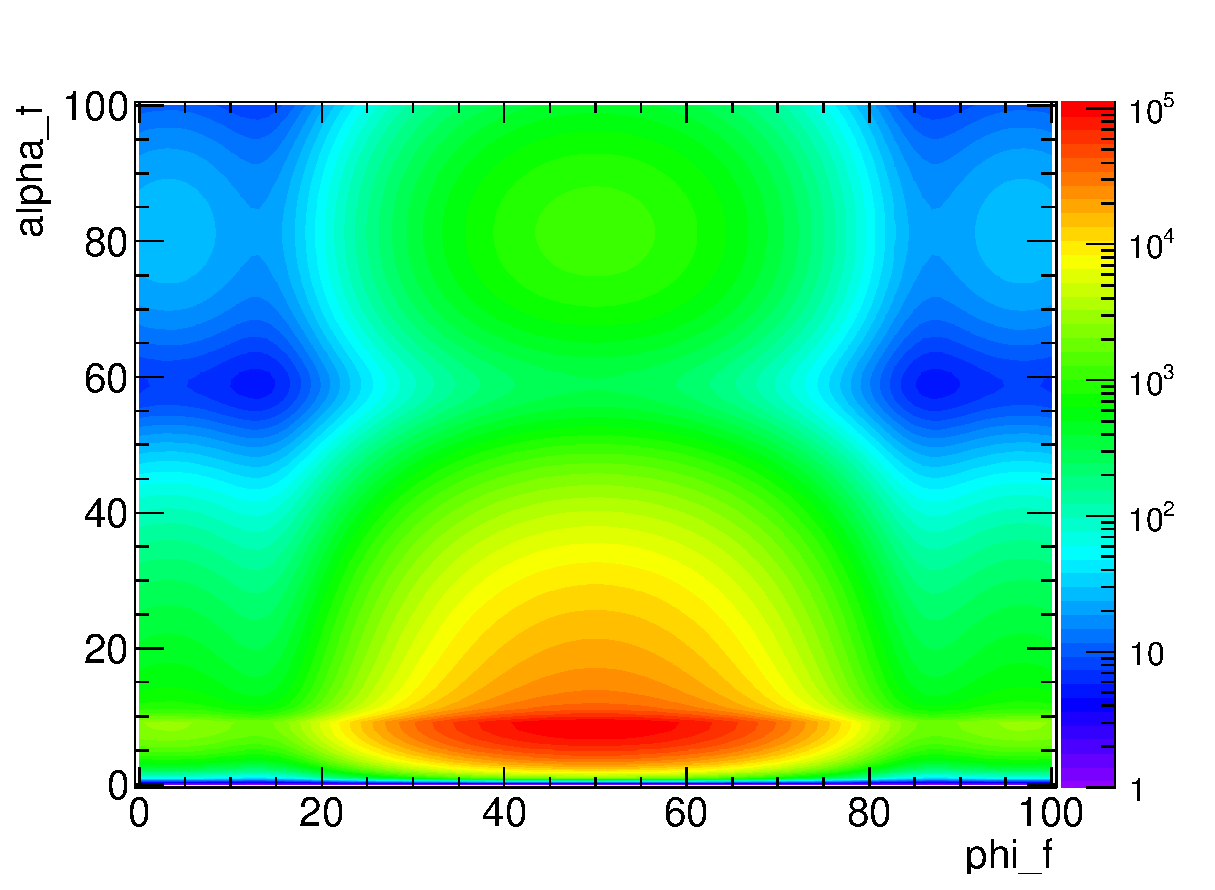
\includegraphics[clip=true, width=120mm]{Figures/Manual_ex1.eps}
  \end{center}
  \caption[Example 1: Simulated grazing-incidence small-angle X-ray scattering from a mixture of
cylindrical and prismatic nanoparticles without any interference, deposited on top
of a substrate]{Figure of example 1: Simulated grazing-incidence small-angle X-ray scattering from a mixture of
cylindrical and prismatic nanoparticles without any interference, deposited on top
of a substrate. The input beam is characterized by a wavelength
$\lambda$ of 1~\AA\ and incident angles $\alpha_i=0.2^{\circ}$, $\phi_i=0^{\circ}$. The
cylinders have a radius and a height both equal to 5~nm, the prisms
are characterized by a side length equal to 5~nm and they are also 5~nm high. The
material of the particles has a refractive index of $1-6\times 10^{-4}+i2\times 10^{-8}$. For the substrate
it is equal to $1-6\times 10^{-6} +i2\times 10^{-8} $. The colorscale
is associated with the output intensity in arbitrary units. }
\label{fig:output_ex1}
\end{figure}



%%%%%%%%%%%%%%%%%%%%%%%%%%%%%%%%%%%%%%%%%%%%%%%%%%%%%%%%%%%%%%%%%%%%%%%%%%%%%%%
%
%%%%%%%%%%%%%%%%%%%%%%%%%%%%%%%%%%%%%%%%%%%%%%%%%%%%%%%%%%%%%%%%%%%%%%%%%%%%%%%
\section{Example 2: working with sample parameters.} \SecLabel{WorkingWithSampleParameters}

This section gives additional details about the manipulation of sample parameters
at run time, that is after the sample has already been constructed. 
For single simulation this is normally not necessary, however it might be useful
during interactive work when user tries to find optimal sample parameters by
running a series of consequent simulations.
Similarly, this task arises when the theoretical model, presented by the sample and the simulation descriptions, is used for the fitting of real data.
In this case fitting kernel has to be informed about existing sample parameters
and has to have a mechanism for changing values of these parameters to find 
they optimal values.

In \BornAgain\ this is done using so called sample parameter pool mechanism 
and we will briefly explain it using example from the previous
\SecRef{Example1Python}.

Inside \BornAgain\ sample is described by a hierarchical tree of objects.
For the multilayer created in previous section this tree can be graphically
represented as shown in Fig.~\ref{fig:sample_tree}. 

\begin{figure}[p!]

\tikzstyle{every node}=[draw=black,thick,anchor=west]
\tikzstyle{selected}=[draw=red,fill=red!30]
\tikzstyle{optional}=[dashed,fill=gray!50]
\begin{tikzpicture}[%
  grow via three points={one child at (0.5,-0.7) and
  two children at (0.5,-0.7) and (0.5,-1.4)},
  edge from parent path={(\tikzparentnode.south) |- (\tikzchildnode.west)}]
  \node {MultiLayer}
    child { node {Layer \#0}
		child { node {ParticleDecoration } 
			child { node {Particle Info 0} 
				child {node {Particle }  
					child { node {FormFactorCylinder} 
						child { node [optional] { height:5.0} }					
						child { node [optional] { radius:5.0} }					
					}				
				}
    			child [missing] {}		
    			child [missing] {}		
			    child [missing] {}		
				child {node [optional] { abundance:0.5} }			
				child {node [optional] { depth:0.0} }			
			}
    		child [missing] {}		
    		child [missing] {}		
			child [missing] {}		
    		child [missing] {}		
    		child [missing] {}		
			child [missing] {}		
			child { node {Particle Info 1} 
				child {node {Particle }  
					child { node {FormFactorPrism3} 
						child { node [optional] { half\_side:5.0} }					
						child { node [optional] { height:5.0} }					
					}				
				}
    			child [missing] {}		
    			child [missing] {}		
			    child [missing] {}		
				child {node [optional] { abundance:0.5} }			
				child {node [optional] { depth:0.0} }						
			}					
		}
		child [missing] {}		
   		child [missing] {}		
	    child [missing] {}		
		child [missing] {}		
   		child [missing] {}		
	    child [missing] {}		
	    child [missing] {}		
		child [missing] {}		
   		child [missing] {}		
	    child [missing] {}		
		child [missing] {}		
   		child [missing] {}		
	    child [missing] {}		
	    child [missing] {}		
		child {node [optional] { thickness:0.0} }				
    }
	child [missing] {}		
   	child [missing] {}		
	child [missing] {}		
   	child [missing] {}		
	child [missing] {}		
	child [missing] {}		
   	child [missing] {}		
	child [missing] {}		
   	child [missing] {}		
	child [missing] {}		
	child [missing] {}		
   	child [missing] {}		
	child [missing] {}		
   	child [missing] {}		
	child [missing] {}		
	child [missing] {}		
	child { node {Layer interface \#0} 
    	child {node { roughness} 
    		child {node [optional] { corrlength:0.0} }				    	
    		child {node [optional] { hurst:0.0} }				    	
    		child {node [optional] { sigma:0.0} }				    	
    	}					
	}
   	child [missing] {}		
	child [missing] {}		
	child [missing] {}		
    child { node {Layer \#1}
    	child {node [optional] { thickness:0.0} }				
    }
	child [missing] {}		
    child { node [optional] {CrossCorrLength:0.0} };
    
\end{tikzpicture}
\caption{Tree representation of the sample structure.}
\label{fig:sample_tree}
\end{figure}


The top \Code{MultiLayer} object is composed of three children, namely
\Code{Layer \#0, Layer Interface \#0} and \Code{Layer \#1}. Children objects
by turn might also be composed into tree-like structure. For example,
\Code{Layer \#0} contains \Code{ParticleDecoration} object which holds all information
related to the particles populating the layer. All numerical values which have been used
during sample construction (thickness of layers, size of particles, roughness parameters) are the part of the same tree structure. 
They are marked in the figure with shaded gray boxes.

These values are registered in the sample parameter pool using the name
composed from the names of corresponding nodes of the tree and can be accessed/changed
during run time. For example, the \Code{height} of the cylinders populating first layer can be changed from 
current $5~nm$ to $1~nm$ by running the command

\begin{lstlisting}[language=shell, style=commandline]
multi_layer.setParameterValue('/MultiLayer/Layer0/ParticleDecoration/ParticleInfo0/Particle/FormFactorCylinder/height', 1.0)
\end{lstlisting}


The user can get names and values of all registered sample's parameters using the command 

\begin{lstlisting}[language=shell, style=commandline]
> multi_layer.printParameters()
The sample contains following parameters ('name':value)
'/MultiLayer/Layer0/ParticleDecoration/ParticleInfo0/Particle/FormFactorCylinder/height':5
'/MultiLayer/Layer0/ParticleDecoration/ParticleInfo0/Particle/FormFactorCylinder/radius':5
'/MultiLayer/Layer0/ParticleDecoration/ParticleInfo0/abundance':0.5
'/MultiLayer/Layer0/ParticleDecoration/ParticleInfo0/depth':0
'/MultiLayer/Layer0/ParticleDecoration/ParticleInfo1/Particle/FormFactorPrism3/half_side':5
'/MultiLayer/Layer0/ParticleDecoration/ParticleInfo1/Particle/FormFactorPrism3/height':5
'/MultiLayer/Layer0/ParticleDecoration/ParticleInfo1/abundance':0.5
'/MultiLayer/Layer0/ParticleDecoration/ParticleInfo1/depth':0
'/MultiLayer/Layer0/thickness':0
'/MultiLayer/Layer1/thickness':0
'/MultiLayer/LayerInterface/roughness/corrlength':0
'/MultiLayer/LayerInterface/roughness/hurst':0
'/MultiLayer/LayerInterface/roughness/sigma':0
'/MultiLayer/crossCorrLength':0
\end{lstlisting}

Wildcards \Code{'*'} can be used to reduce typing or to work on group of parameters. In example below first command will change the height of the cylinders in the same way, as in previous example, while the second line will change the depth of both cylinders and prisms.
\begin{lstlisting}[language=shell, style=commandline]
multi_layer.setParameterValue('*FormFactorCylinder/height', 1.0)
multi_layer.setParameterValue('*depth', 1.0)
\end{lstlisting}

The complete example to this section can be found at
\begin{lstlisting}[language=shell, style=commandline]
./Examples/python/fitting/ex001_SampleParametersIntro.py
\end{lstlisting}






%\section{Basic Python fitting example/}

%%%%%%%%%%%%%%%%%%%%%%%%%%%%%%%%%%%%%%%%%%%%%%%%%%%%%%%%%%%%%%%%%%%%%%%%%%%%%%%%
%%
%%   BornAgain User Manual
%%
%%   homepage:   http://www.bornagainproject.org
%%
%%   copyright:  Forschungszentrum Jülich GmbH 2015
%%
%%   license:    Creative Commons CC-BY-SA
%%   
%%   authors:    Scientific Computing Group at MLZ Garching
%%               C. Durniak, M. Ganeva, G. Pospelov, W. Van Herck, J. Wuttke
%%
%%%%%%%%%%%%%%%%%%%%%%%%%%%%%%%%%%%%%%%%%%%%%%%%%%%%%%%%%%%%%%%%%%%%%%%%%%%%%%%%


\newpage
\chapter{Software architecture}\SecLabel{SoftwareArchitecture}
 

%%%%%%%%%%%%%%%%%%%%%%%%%%%%%%%%%%%%%%%%%%%%%%%%%%%%%%%%%%%%%%%%%%%%%%%%%%%%%%%%
\section{Basic structure of \BornAgain}
%%%%%%%%%%%%%%%%%%%%%%%%%%%%%%%%%%%%%%%%%%%%%%%%%%%%%%%%%%%%%%%%%%%%%%%%%%%%%%%%

\BornAgain\ is written in \Code{C++}
and uses an object oriented approach to 
achieve modularity, extensibility and transparency.
This leads to the task driven rather than the command driven approach in 
different aspects of the simulation and fitting of GISAS data.
The user defines the sample structure, beam and detector characteristics and
fit parameters using building
blocks -- \Code{classes} -- defined in core libraries of the framework.
These buildings blocks are combined by the user according to his current
task using one the following approaches:
\begin{itemize}
\item The user creates a \Python\ script with a sample description and simulation settings
using the \BornAgain\ API.
The user then runs the simulation by executing the script in the \Python\ interpreter and assesses the
simulation results using his preferred graphics or analysis library, e.g. \Python\ + \Code{numpy} + \Code{matplotlib}.
\item The user may write a standalone \Code{C++} application linked to the \BornAgain\ libraries.
\item The user interacts with the framework through a graphical 
user interface (forthcoming).
\end{itemize}

The object oriented approach in the software design allows users 
to have a much higher level of flexibility in the sample construction; it also
decouples the building blocks used in the internal calculations and thereby facilitates the creation of new models,
with little or no modification to the existing code. 


\begin{figure}[htbp]
\centering
  \resizebox{0.9\textwidth}{!}{%
    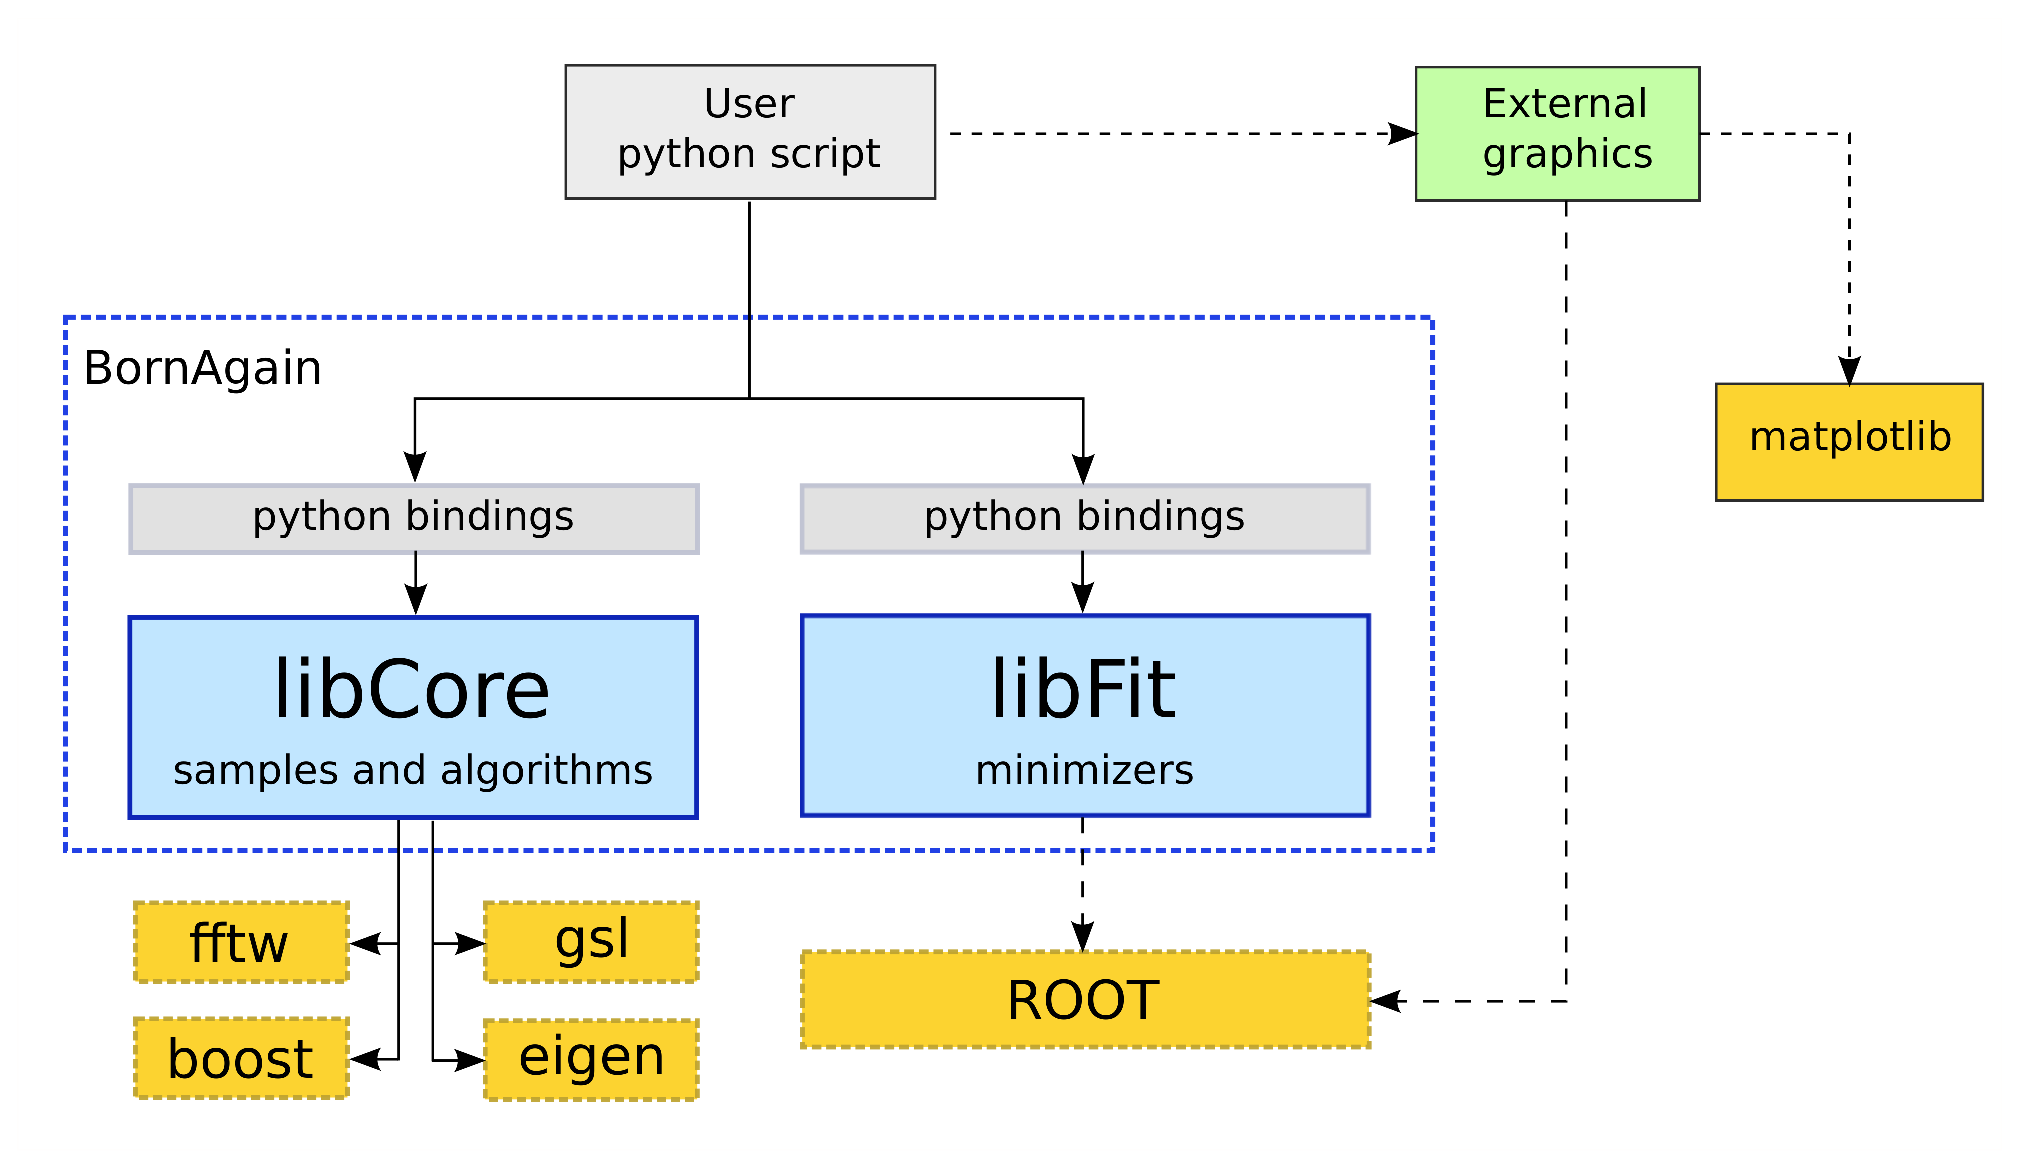
\includegraphics{fig/drawing/basic_architecture.eps}}
\caption{Structure of \BornAgain\ libraries.}
\label{fig:two_ratios}
\end{figure}


The general structure of \BornAgain\ and the way the user interacts with it are
shown in Fig.~\ref{fig:two_ratios}.
The framework consists of two shared libraries, \Code{libBornAgainCore} and
\Code{libBornAgainFit}. Thanks to the \Python\ interface they can be imported into \Python\ as external modules. The library \Code{libBornAgainCore} contains a number of classes, grouped into several class categories, necessary for the description of a model and running a simulation.
The library  \Code{libBornAgainFit} contains a number of minimization engines 
and interfaces to them, allowing the user to fit real data with the model previously defined.

\BornAgain\ depends on a few external and well established
open-source libraries: \Code{boost}, GNU scientific library, Eigen and
Fast Fourier Transformation libraries. They are required to be
installed on the system to run \BornAgain\ on Unix Platforms. In the
case of Windows Platform they are added to the system automatically during \BornAgain\ installation. Other libraries shown
on the plot (\Code{ROOT}, \Code{matplotlib}) are optional.

 
%%%%%%%%%%%%%%%%%%%%%%%%%%%%%%%%%%%%%%%%%%%%%%%%%%%%%%%%%%%%%%%%%%%%%%%%%%%%%%%%
\section{Data classes for simulations and fits}
%%%%%%%%%%%%%%%%%%%%%%%%%%%%%%%%%%%%%%%%%%%%%%%%%%%%%%%%%%%%%%%%%%%%%%%%%%%%%%%%

This section will give an overview of the classes that are used to describe all the data needed to perform a single simulation. The prime elements of this data are formed by the sample, the experimental conditions (beam and detector parameters) and simulation parameters.

These classes constitute the main interface to the software's users, since they will mostly be interacting with the program by creating samples and running simulations with specific parameters. Since it is not the intent to explain internals of classes in this document, the text and figures will only mention the most important methods and fields of the classes discussed. Furthermore, getters and setters of private member fields will not be indicated, although these do belong to the public interface. For more detailed information about the project's classes, their methods and fields, the reader is referred to the source code documentation. REF?



\subsection{The Experiment object}
The \Code{Experiment} class holds all references to data objects that are needed to perform a simulation. These consist in a sample description, possibly implemented by a builder object, detector and beam parameters and finally, a simulation parameter class that defines the different approximations that can be used during a simulation. Besides getters and setters for these fields, the class also contains a \Code{runSimulation()} method that will generate an ISimulation object that will perform the actual computations. The class diagram for \Code{Experiment} is shown in \reffig{exp}.

\vspace{8mm}
\begin{figure}[H]
%the makebox macro ensures centering of the resulting figure
\makebox[\textwidth][c]{
\begin{tikzpicture}
\begin{umlpackage}{Simulation Data}
\umlclass{Experiment}{
  -- mp\_sample : ISample* \\
  -- mp\_sample\_builder : ISampleBuilder* \\
  -- m\_detector : Detector \\
  -- m\_beam : Beam \\
  -- m\_intensity\_map : OutputData<double> \\
  -- m\_sim\_params : SimulationParameters
}{
  \umlvirt{+ clone() : Experiment*} \\
  \umlvirt{+ runSimulation() : void} \\
  \umlvirt{+ normalize() : void}
}
\umlemptyclass[x=7, y=0]{ISample}
\umlemptyclass[x=7, y=-2]{Detector}
\umlemptyclass[x=7, y=-4]{Beam}
\umlemptyclass[x=7, y=-6]{SimulationParameters}
\umlemptyclass[y=-4]{GISASExperiment}
\umluniassoc[geometry=|-, anchor1=0]{Experiment}{ISample}
\umluniassoc[geometry=|-, anchor1=0]{Experiment}{Detector}
\umluniassoc[geometry=|-, anchor1=0]{Experiment}{Beam}
\umluniassoc[geometry=|-, anchor1=0]{Experiment}{SimulationParameters}
\umlinherit[geometry=--]{GISASExperiment}{Experiment}

\umlnote[y=-6.5, width=6cm]{GISASExperiment}{
  The ``runSimulation()'' method retrieves an ISimulation object
  from the topmost ISample object and calls its ``run()'' method 
  to perform the actual computations.
}
\end{umlpackage}
\end{tikzpicture}
} %end makebox
\caption{The Experiment class as a container for sample, beam, detector and simulation parameters.}
\label{fig:exp}
\end{figure}

\subsection{The ISample class hierarchy}

Samples are described by a hierarchical tree of objects which all adhere to the ISample interface. The composite pattern is used to achieve a common interface for all objects in the sample tree. The sample description is maximally decoupled from all computational classes, with the exception of the ``createDWBASimulation()'' method. This method will create a new object of type ``DWBASimulation'' that is capable of calculating the scattering contributions originating from the sample part in question. This coupling is not very tight however, since the ISample subclasses only need to know about which class to instantiate and return.

This interface and two of its subclasses are sketched in \reffig{isample}.

\vspace{8mm}

\begin{figure}[H]
\makebox[\textwidth][c]{
\begin{tikzpicture}
\begin{umlpackage}{Sample description} 
% Code from official documentation goes here...
\umlinterface{ISample}{
}{
  \umlvirt{+ clone() : ISample*} \\
  \umlvirt{+ createDWBASimulation() : DWBASimulation*}
}
\umlclass[y=-4]{MultiLayer}{
  -- m\_layers : std::vector<Layer *> \\
  -- m\_interfaces : std::vector<LayerInterface *>
}{
  + getNumberOfLayers() : size\_t \\
  + getNumberOfInterfaces() : size\_t \\
  + addLayer(const Layer \&layer) : void
}
\umlclass[x=8,y=-4]{Layer}{
  -- mp\_material : IMaterial* \\
  -- m\_thickness : double
}{
  + getThickness() : double \\
  + setThickness(double thickness) : void
}
\umlinherit[geometry=-|]{MultiLayer}{ISample}
\umlinherit[geometry=|-]{Layer}{ISample}
\umluniassoc[geometry=--, mult2=n]{MultiLayer}{Layer}
\end{umlpackage}
\end{tikzpicture}
}
\caption{The ISample interface}
\label{fig:isample}
\end{figure}



\subsection{The FitSuite class} \SecLabel{FitSuiteClass}

\subsection{The IMinimizer class} \SecLabel{IMinimizerClass}

\subsection{The MinimizerOptions class} \SecLabel{MinimizerOptionsClass}

%\input{SoftwareDesignOverview}
%\appendix
%\newpage{\pagestyle{empty}\cleardoublepage}


%\mychapter{1}{Appendix}

\chapter{Listings}

\begin{lstlisting}[caption={Python script of example 1},
  label=script_ex1,captionpos=b,escapeinside={@}{@} ,language=python,style=eclipse, numbers= none,frame = leftline ,
      framerule = 2mm ,
      rulecolor = \color{lightgrey},
      breaklines = true]
import sys, os, numpy 

sys.path.append(os.path.abspath(os.path.join(os.path.split(__file__)[0],'..', '..', '..', 'lib')))

from libBornAgainCore import * 

def RunSimulation():
    #  defining materials 
    mAmbience = MaterialManager.getHomogeneousMaterial("Air", 0.0, 0.0 ) 
    mSubstrate = MaterialManager.getHomogeneousMaterial("Substrate",
    6e-6, 2e-8) 
    mParticle = MaterialManager.getHomogeneousMaterial("Particle", 6e-4, 2e-8 )
    # collection of particles 
    cylinder_ff = FormFactorCylinder(5*nanometer, 5*nanometer) 
    cylinder = Particle(mParticle, cylinder_ff) 
    prism_ff = FormFactorPrism3(5*nanometer, 5*nanometer) 
    prism = Particle(mParticle, prism_ff) 
    particle_decoration = ParticleDecoration()  
    particle_decoration.addParticle(cylinder, 0.0, 0.5)  
    particle_decoration.addParticle(prism, 0.0, 0.5)  
    interference = InterferenceFunctionNone()  
    particle_decoration.addInterferenceFunction(interference)  
    # air layer with particles and substrate form multi layer 
    air_layer = Layer(mAmbience)  
    air_layer.setDecoration(particle_decoration)
    substrate_layer = Layer(mSubstrate, 0) 
    multi_layer = MultiLayer()  
    multi_layer.addLayer(air_layer) 
    multi_layer.addLayer(substrate_layer) 

    # build and run simulation  
    simulation = Simulation()  
    simulation.setDetectorParameters(100,-1.0*degree, 1.0*degree, 
                                    100, 0.0*degree, 2.0*degree, True) 
    simulation.setBeamParameters(1.0*angstrom, 0.2*degree, 0.0*degree) 
    simulation.setSample(multi_layer) 
    simulation.runSimulation()  

    # retrieving intensity data
     return GetOutputData(simulation)
\end{lstlisting}


\begin{lstlisting}[caption={Python script of fitting example},
  label=script_exfit1,captionpos=b,escapeinside={@}{@} ,language=python,style=eclipse, numbers= none,frame = leftline ,
      framerule = 2mm ,
      rulecolor = \color{lightgrey},
      breaklines = true]
import sys, os, numpy
import math 

sys.path.append(os.path.abspath(
                os.path.join(os.path.split(__file__)[0],
                '..', '..', '..', 'lib')))

from libBornAgainCore import *
from libBornAgainFit import *

# values we want to find
cylinder_height = 5.0*nanometer
cylinder_radius = 5.0*nanometer
prism3_half_side = 5.0*nanometer
prism3_height = 5.0*nanometer
# ----------------------------------
# create sample : cylinders and prisms in the air on substrate layer
# ----------------------------------
def buildSample(): 
    # defining materials
    mAmbience = MaterialManager.getHomogeneousMaterial("Air", 0.0, 0.0 )
    mSubstrate = MaterialManager.getHomogeneousMaterial("Substrate",
    6e-6, 2e-8 )
    mParticle = MaterialManager.getHomogeneousMaterial("Particle", 6e-4, 2e-8 )
    # collection of particles
    cylinder_ff = FormFactorCylinder(cylinder_height, cylinder_radius)
    cylinder = Particle(mParticle, cylinder_ff)
    prism_ff = FormFactorPrism3(prism3_height,  prism3_half_side)
    prism = Particle(mParticle, prism_ff)
    particle_decoration = ParticleDecoration()
    particle_decoration.addParticle(cylinder, 0.0, 0.5)
    particle_decoration.addParticle(prism,0.0, 0.5)  
    interference = InterferenceFunctionNone()
    particle_decoration.addInterferenceFunction(interference)
    # air layer with particles and substrate form multi layer
    air_layer = Layer(mAmbience)
    air_layer.setDecoration(particle_decoration)
    substrate_layer = Layer(mSubstrate, 0)
    multi_layer = MultiLayer()
    multi_layer.addLayer(air_layer)
    multi_layer.addLayer(substrate_layer)
    return multi_layer
# ----------------------------------
# create sample : input beam and detector - characteristics
# ----------------------------------
def createSimulation():
    simulation = Simulation()
    simulation.setDetectorParameters(100, 0.0*degree, 2.0*degree,100 , 0.0*degree, 2.0*degree)
    simulation.setBeamParameters(1.0*angstrom, 0.2*degree, 0.0*degree)
    return simulation
# ----------------------------------
# read "real" data from file
# ----------------------------------
def GetRealData():
    real_data = OutputDataIOFactory.getOutputData('Refdata_fitcylinderprisms.txt')
    return real_data
# ----------------------------------
# run fitting 
# ----------------------------------
def run_fitting():
    sample = buildSample()
    simulation = createSimulation()
    simulation.setSample(sample)
    # get the real data, which is simply results of our simulation with default values
    real_data = GetRealData()   
    # run the simulation
    simulation.runSimulation()    
    # linking real and numerical (to be fitted) data
    fitSuite = FitSuite()
    fitSuite.addSimulationAndRealData(simulation, real_data)  
    # setting fitting minimizer
    fitSuite.setMinimizer( MinimizerFactory.createMinimizer("Minuit2","Migrad") ) 
    # setting fitting parameters
    fitSuite.addFitParameter("*FormFactorCylinder/height", 4.*nanometer, 0.01*nanometer, AttLimits.lowerLimited(0.01) )
    fitSuite.addFitParameter("*FormFactorCylinder/radius", 6.*nanometer, 0.01*nanometer, AttLimits.lowerLimited(0.01) )
    fitSuite.addFitParameter("*FormFactorPrism3/height", 4.*nanometer, 0.01*nanometer, AttLimits.lowerLimited(0.01) )
    fitSuite.addFitParameter("*FormFactorPrism3/half_side", 6*nanometer, 0.01*nanometer, AttLimits.lowerLimited(0.01) )
    # run fit
    fitSuite.runFit()
    # print fit results
    fitSuite.printResults()
\end{lstlisting}


%%Appendix
\chapter{Implemented classes}

\begin{itemize}
\item Particle decoration
\item Layer
\item MultiLayer
\item Simulation
\end{itemize}

\chapter{Form factors}
% plots of particles + orientation of the axes
% plots of the form factors

\begin{itemize}
\item Parallelepiped (\texttt{FormFactorParallelepiped})

\begin{equation}
F(\mathbf{q},R, H) = 4H R^2\exp(i q_z H/2) \text{sinc}(q_xR)
\text{sinc}(q_yR)\text{sinc}(q_z H/2)
\end{equation}
%%%%%%%%%%%%%%%%%%%%%%%%%%%%%%%%%%%
\item Pyramid (\texttt{FormFactorPyramid})

\begin{align*}
        q_1 &=\frac{1}{2}\Big[\frac{q_x-q_y}{\tan(\alpha)} + q_z\Big],\quad       q_2 =\frac{1}{2}\Big[\frac{q_x-q_y}{\tan(\alpha)} - q_z\Big]\quad
        q_3 =\frac{1}{2}\Big[\frac{q_x+q_y}{\tan(\alpha)} + q_z\Big]\quad       q_4 =\frac{1}{2}\Big[\frac{q_x+q_y}{\tan(\alpha)} - q_z\Big]\\
        K_1 &= \text{sinc}(q_1 H)\exp(i q_1 H)  + i \text{sinc}(q_2 H) \exp(-i q_2 H)\\
        K_2 &= -i \text{sinc}(q_1 H) \exp(i q_1 H) +i
        \text{sinc}(q_2 H) \exp(-i q_2 H)\\
        K_3 &= \text{sinc}(q_3 H) \exp(i q_3 H)    +
        \text{sinc}(q_4 H) \exp(-i q_4 H)\\
        K_4 &= -i \text{sinc}(q_3 H) \exp(i q_3 H) + i \text{sinc}(q_4 H) \exp(-i q_4 H)\\     
  F(\mathbf{q},R, H, \alpha) &= \frac{H}{q_x q_y} \Big\{ K_1 \cos[ (q_x-q_y)R ] + K_2 \sin[ (q_x-q_y)R ] - K_3 \cos[ (q_x+q_y) R ] - K_4 \sin[ (q_x+q_y) R ]\Big\}
   \end{align*}
%%%%%%%%%%%%%%%%%%%%%%%%%%%%%%%%%%%%	
\item Cylinder (\texttt{FormFactorCylinder})

  \begin{equation}
 F(\mathbf{q},R, H)=   H  \text{sinc}(q_ z H/2) \exp(i q_ z H/2) 2\pi R^2 \frac{J_1(|q_{\parallel} R |)}{|q_{\parallel} R| }
 \end{equation}
 
%%%%%%%%%%%%%%%%%%%%%%%%%%%%%%%%%%%%
\item Prism3 (\texttt{FormFactorPrism3})

\begin{align*}
    F(\mathbf{q},R, H) &= 2 \sqrt{3}\frac{\exp(-i q_y
      R/\sqrt{3})}{q_x^2-3q_y^2} \Big[\exp(i \sqrt{3} q_y R )
    -\cos(q_x R)-i \sqrt{3} q_y R \text{sinc}(q_x R) \Big] \\
   &\times  H \text{sinc}(q_z H/2 ) \exp(i q_z H/2)
\end{align*}

%%%%%%%%%%%%%%%%%%%%%%%%%%%%%%%%%%%%
\item Sphere (\texttt{FormFactorSphere})

\begin{equation}    
F(\mathbf{q},R, H)= 2\pi \exp[i q_z (H-R)]\int_{R-H} ^{R} R_z^2 \frac{J_1(|q_{\parallel}
  R_z|) }{|q_{\parallel} R_z|}
        \exp(i q_z z) dz
\end{equation}

$R_z=\sqrt{R^2-z^2}$, $q_{\parallel}=\sqrt{q_x^2+q_y^2}$

%%%%%%%%%%%%%%%%%%%%%%%%%%%%%%%%%%%%
\item Full sphere (\texttt{FormFactorFullSphere})

\begin{equation}
F(\mathbf{q},R) = 4\pi R^3 \frac{\sin(q R) - q R \cos(q R)}{(qR)^3}
\end{equation}
%%%%%%%%%%%%%%%%%%%%%%%%%%%%%%%%%%%%
\item Box (\texttt{FormFactorBox})

\begin{equation}
F(\mathbf{q},R,W,H)= 4H R W\exp(i q_z H/2) \text{sinc}(q_x R) \text{sinc}(q_y W) \text{sinc}(q_z H/2)
\end{equation}
    
where $\text{sinc}(x)=\sin(x)/x$ is the cardinal sine, $J_1(x)$ is the
Bessel function of first order.
	
\end{itemize}

\chapter{Interference functions}

\begin{itemize}
\item	No interference 
\item	decoupling approximation 	
\item 	local mono disperse approximation 
\item 	size spacing approximation 
\end{itemize}


\chapter{Pair correlation functions}
\begin{itemize}
\item The Debye hard core 
\item The gaussian
\item The Lennard-Jones  	
\item The gate pair correlation 	
\item The Debye hard core with power-law decrease  	
\item The Zhu pair correlation function 	
\item The Venables pair correlation function 	
\item The bidimensional hard core pair function.
\end{itemize}	


%\bibliographystyle{switch}
\bibliographystyle{unsrt}
\bibliography{jw7}

\end{document}
